\begin{tikzpicture}[
	every axis/.style={
		%grid=major,
		%grid style={dotted},
		ybar stacked,
		%ylabel={"Time [s]"},
		%ymode=log,
		%ymin=0,ymax=15,
		y tick label style={
			font=\footnotesize
		},
		x tick label style={
			% add some negative yshift to move ticklabels down
			yshift=-2mm,
			rotate=45,
			anchor=east,
			font=\scriptsize
		},
		%x axis line style = { opacity = 0 }, 
		%y axis line style = { opacity = 0 },
		tickwidth = 0pt,
		width=0.5\textwidth,
		height=0.3\textheight,
		% symbolic coords have numerical distance of 1
		% so with the following line you get a tick at every symbolic coord
		xtick distance=1,
		symbolic x coords={CESM-ATM,ISABEL,NYX,SCALE-LETKF,QMCPACK,Miranda,S3D,EXAFEL},
		bar width=2pt
	},
	]
	\pgfplotsset{
		% define a new style used for the plot used to add labels
		% 2 args means it takes two mandatory arguments, so must be used as
		% labelplot={first arg}{second arg}
		labelplot/.style 2 args={
			% forget plot means it doesn't affect cycle lists or legends
			forget plot,
			% #1 is first argument, the text used in the nodes near coords
			nodes near coords=#1,
			% #2 is second argument, a length that should be the same as the bar shift for the axis
			every node near coord/.style={below,font=\tiny,xshift=#2}
		}
	}
	
	\begin{axis}[bar shift=-9pt,grid=major,grid style={dotted},ylabel={Time [s]},ymin=0,ymax=15,yticklabels={0,5,10,15},ytick={0,5,10,15}] % tlib
		\addplot [labelplot={1st}{-9pt}] coordinates {(CESM-ATM,0) (ISABEL,0) (NYX,0) (SCALE-LETKF,0) (QMCPACK,0) (Miranda,0) (S3D,0) (EXAFEL,0)};
		\addplot+[fill=blue!30!white] coordinates { (CESM-ATM,0.840) (ISABEL,0.134) (NYX,0.263) (SCALE-LETKF,1.229) (QMCPACK,0.023) (Miranda,0.032) (S3D,0.204) (EXAFEL,0.141) };
		\addplot+[fill=red!30!white] coordinates { (CESM-ATM,0.010) (ISABEL,0.020) (NYX,0.149) (SCALE-LETKF,0.099) (QMCPACK,0.072) (Miranda,0.027) (S3D,0.237) (EXAFEL,1.992) };
		\addplot+[fill=yellow!30!white] coordinates { (CESM-ATM,0.006) (ISABEL,0.021) (NYX,0.149) (SCALE-LETKF,0.114) (QMCPACK,0.010) (Miranda,0.030) (S3D,0.311) (EXAFEL,1.636) };
		\addplot+[fill=green!30!white] coordinates { (CESM-ATM,0.004) (ISABEL,0.185) (NYX,3.591) (SCALE-LETKF,1.053) (QMCPACK,0.015) (Miranda,0.800) (S3D,2.192) (EXAFEL,0.826) };
	\end{axis}
	
	\begin{axis}[bar shift=-6pt, xticklabels={},ymin=0,ymax=15,yticklabels={}] % tuckermpi
		\addplot [labelplot={2nd}{-3pt}]coordinates {(CESM-ATM,0) (ISABEL,0) (NYX,0) (SCALE-LETKF,0) (QMCPACK,0) (Miranda,0) (S3D,0) (EXAFEL,0)};
		\addplot+[fill=blue!30!white] coordinates { (CESM-ATM,0) (ISABEL,0) (NYX,0) (SCALE-LETKF,0) (QMCPACK,0) (Miranda,0) (S3D,0) (EXAFEL,0) };
		\addplot+[fill=red!30!white] coordinates { (CESM-ATM,0) (ISABEL,0) (NYX,0) (SCALE-LETKF,0) (QMCPACK,0) (Miranda,0) (S3D,0) (EXAFEL,0) };
		\addplot+[fill=yellow!30!white] coordinates { (CESM-ATM,0) (ISABEL,0) (NYX,0) (SCALE-LETKF,0) (QMCPACK,0) (Miranda,0) (S3D,0) (EXAFEL,0) };
		\addplot+[fill=green!30!white] coordinates { (CESM-ATM,0) (ISABEL,0) (NYX,0) (SCALE-LETKF,0) (QMCPACK,0) (Miranda,0) (S3D,0) (EXAFEL,0) };
	\end{axis}
	
	\begin{axis}[bar shift=-3pt,xticklabels={},ymin=0,ymax=15,yticklabels={}] % tblis
		\addplot+[fill=blue!30!white] coordinates { (CESM-ATM,0.878) (ISABEL,0.158) (NYX,0.200) (SCALE-LETKF,1.447) (QMCPACK,0.016) (Miranda,0.056) (S3D,0.240) (EXAFEL,0.318) };
		\addplot+[fill=red!30!white] coordinates { (CESM-ATM,0.009) (ISABEL,0.030) (NYX,0.201) (SCALE-LETKF,0.139) (QMCPACK,0.015) (Miranda,0.044) (S3D,0.324) (EXAFEL,2.678) };
		\addplot+[fill=yellow!30!white] coordinates { (CESM-ATM,0.009) (ISABEL,0.031) (NYX,0.395) (SCALE-LETKF,0.139) (QMCPACK,0.017) (Miranda,0.048) (S3D,0.360) (EXAFEL,1.256) };
		\addplot+[fill=green!30!white] coordinates { (CESM-ATM,0.006) (ISABEL,0.503) (NYX,3.837) (SCALE-LETKF,1.272) (QMCPACK,0.083) (Miranda,1.043) (S3D,3.878) (EXAFEL,2.088) };
	\end{axis}
	
	\begin{axis}[bar shift=0pt,xticklabels={},ymin=0,ymax=15,yticklabels={}] % tcl
		\addplot+[fill=blue!30!white] coordinates { (CESM-ATM,0.783) (ISABEL,0.165) (NYX,0.248) (SCALE-LETKF,1.590) (QMCPACK,0.017) (Miranda,0.050) (S3D,0.288) (EXAFEL,0.000) };
		\addplot+[fill=red!30!white] coordinates { (CESM-ATM,0.027) (ISABEL,0.044) (NYX,0.210) (SCALE-LETKF,0.182) (QMCPACK,0.017) (Miranda,0.049) (S3D,0.343) (EXAFEL,0.000) };
		\addplot+[fill=yellow!30!white] coordinates { (CESM-ATM,0.003) (ISABEL,0.030) (NYX,0.203) (SCALE-LETKF,0.135) (QMCPACK,0.023) (Miranda,0.040) (S3D,0.367) (EXAFEL,0.000) };
		\addplot+[fill=green!30!white] coordinates { (CESM-ATM,0.003) (ISABEL,0.078) (NYX,2.625) (SCALE-LETKF,0.307) (QMCPACK,0.014) (Miranda,0.229) (S3D,1.419) (EXAFEL,0.000) };
	\end{axis}
	
	\begin{axis}[bar shift=3pt,xticklabels={},ymin=0,ymax=15,yticklabels={}] % eigen
		\addplot+[fill=blue!30!white] coordinates { (CESM-ATM,1.009) (ISABEL,0.431) (NYX,0.479) (SCALE-LETKF,3.647) (QMCPACK,0.061) (Miranda,0.207) (S3D,1.319) (EXAFEL,0.295) };
		\addplot+[fill=red!30!white] coordinates { (CESM-ATM,0.017) (ISABEL,0.070) (NYX,0.750) (SCALE-LETKF,0.349) (QMCPACK,0.054) (Miranda,0.101) (S3D,1.175) (EXAFEL,5.663) };
		\addplot+[fill=yellow!30!white] coordinates { (CESM-ATM,0.011) (ISABEL,0.081) (NYX,0.746) (SCALE-LETKF,0.331) (QMCPACK,0.047) (Miranda,0.133) (S3D,1.211) (EXAFEL,4.537) };
		\addplot+[fill=green!30!white] coordinates { (CESM-ATM,0.011) (ISABEL,0.311) (NYX,6.294) (SCALE-LETKF,1.516) (QMCPACK,0.039) (Miranda,0.786) (S3D,3.767) (EXAFEL,3.641) };
	\end{axis}
	
	\begin{axis}[bar shift=6pt,xticklabels={},ymin=0,ymax=15,yticklabels={}] % torch
		\addplot+[fill=blue!30!white] coordinates { (CESM-ATM,0.520) (ISABEL,0.196) (NYX,0.372) (SCALE-LETKF,1.327) (QMCPACK,0.069) (Miranda,0.170) (S3D,0.625) (EXAFEL,0.246) };
		\addplot+[fill=red!30!white] coordinates { (CESM-ATM,0.068) (ISABEL,0.234) (NYX,0.563) (SCALE-LETKF,0.584) (QMCPACK,0.127) (Miranda,0.208) (S3D,0.887) (EXAFEL,5.803) };
		\addplot+[fill=yellow!30!white] coordinates { (CESM-ATM,0.022) (ISABEL,0.227) (NYX,0.478) (SCALE-LETKF,0.543) (QMCPACK,0.105) (Miranda,0.223) (S3D,0.911) (EXAFEL,2.002) };
		\addplot+[fill=green!30!white] coordinates { (CESM-ATM,0.020) (ISABEL,0.259) (NYX,2.856) (SCALE-LETKF,1.493) (QMCPACK,0.044) (Miranda,0.406) (S3D,4.470) (EXAFEL,1.825) };
	\end{axis}	
	
	%\begin{axis}[bar shift=6pt,xticklabels={},ymin=0,ymax=15,yticklabels={}]
	%	\addplot [labelplot={4rd}{6pt}] coordinates {(CESM-ATM,0)     (ISABEL,0)     (NYX,0)      (SCALE-LETKF,0)      (QMCPACK,0) (Miranda,0) (S3D,0) (EXAFEL,0)};
	%	\addplot+[fill=blue!30!white] coordinates { (CESM-ATM,9.233) (ISABEL,2.957) (NYX,5.293) (SCALE-LETKF,35.131) (QMCPACK,0.276) (Miranda,1.402) (S3D,8.675) (EXAFEL,2.351) };
	%	\addplot+[fill=red!30!white] coordinates { (CESM-ATM,0.131) (ISABEL,0.681) (NYX,4.997) (SCALE-LETKF,3.554) (QMCPACK,0.296) (Miranda,0.912) (S3D,8.931) (EXAFEL,71.757) };
	%	\addplot+[fill=yellow!30!white] coordinates { (CESM-ATM,0.099) (ISABEL,0.666) (NYX,4.926) (SCALE-LETKF,3.544) (QMCPACK,0.265) (Miranda,0.904) (S3D,8.883) (EXAFEL,30.443) };
	%	\addplot+[fill=green!30!white] coordinates { (CESM-ATM,0.100) (ISABEL,2.195) (NYX,50.854) (SCALE-LETKF,12.268) (QMCPACK,0.206) (Miranda,6.696) (S3D,49.788) (EXAFEL,27.820) };
	%\end{axis}
	
	
\end{tikzpicture}
